\section{Propulsion and Steering}
\label{sec:propulsion}

The Loon-E utilizes a hybrid propulsion system designed for both high-speed transit and precise station-keeping. This is achieved through a combination of differential thrust and physical rudders.

\subsection{Thruster Configuration}
The vehicle is equipped with two Blue Robotics T200 thrusters mounted at the stern. To maximize performance, these thrusters are powered at 20V via a dedicated battery system. 

\begin{itemize}
    \item \textbf{Power Consumption:} 551 W per propeller at maximum setting.
    \item \textbf{Thrust Output:} Approximately 12.5 kgf of joint thrust.
    \item \textbf{Control Method:} Differential thrust via Electronic Speed Controllers (ESCs).
\end{itemize}

\subsection{Rudder System}
For enhanced maneuverability, physical rudders are positioned directly behind each propeller. While each rudder is actuated by an independent servo motor, they are controlled via a single synchronized signal to reduce the complexity of the propulsion state space.

Based on empirical testing of various profiles (including triangle and oval), a \textbf{fishtail profile} was selected for its superior force production. The system utilizes three discrete positions:
\begin{itemize}
    \item \textbf{Neutral:} $0^{\circ}$
    \item \textbf{Port/Starboard:} $\pm35^{\circ}$ (determined to be the optimal stall angle).
\end{itemize}

\subsection{Control Logic and PID}
The propulsion logic is managed by the \texttt{Control Node}, which implements a Proportional-Integral-Derivative (PID) algorithm to minimize heading error.

\begin{enumerate}
    \item \textbf{Differential Thrust:} During a turn, the outside thruster is set to the maximum PWM value. The speed of the inside thruster is adjusted proportionally to the heading error as calculated by the PID controller.
    \item \textbf{Rudder Engagement:} The rudders remain neutral during minor corrections and only activate when the difference between the current heading and target heading exceeds a pre-defined threshold.
    \item \textbf{Speed Regulation:} The base power of both propellers is scaled proportionally to approach the desired target speed.
\end{enumerate}

\begin{figure}[H]
    \centering
    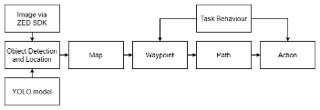
\includegraphics[width=0.8\textwidth]{images/control_flow.png}
    \caption{Control Flow for Thruster and Rudder Coordination}
    \label{fig:propulsion-logic}
\end{figure}